%-------------------------------------------------------------------------
% PACKAGES AND DOCUMENT CONFIGURATIONS
%-------------------------------------------------------------------------

\documentclass[dvipsnames,cmyk]{article}
\usepackage[a4paper, total={7in, 10in}]{geometry}
\usepackage{graphicx}
\usepackage{natbib}
\usepackage{amsmath}
\usepackage[spanish]{babel}
\usepackage[utf8]{inputenc}
\usepackage{courier}
\usepackage{color}
\usepackage{listings}
\usepackage{caption}
\usepackage{subcaption}
\usepackage{hyperref}
\usepackage{booktabs}

\setlength\parindent{0pt}
\renewcommand{\lstlistingname}{Algoritmo}

\usepackage{listings,xcolor}

\lstset{
    breaklines=true,
    tabsize=3,
    showstringspaces=false
}

\lstdefinestyle{Common}{
    extendedchars=\true,
    language={python},
    frame=single,
    framesep=3pt,
    framerule=0.4pt,
    xleftmargin=3.4pt,
    xrightmargin=3.4pt,
    rulecolor=\color{Red}
}

\lstdefinestyle{A}{
    style=Common,
    backgroundcolor=\color{Yellow!10},
    basicstyle=\scriptsize\color{Black}\ttfamily,
    keywordstyle=\color{Orange},
    identifierstyle=\color{Cyan},
    stringstyle=\color{Red},
    commentstyle=\color{Green}
}

\lstdefinestyle{B}{
    style=Common,
    backgroundcolor=\color{Black},
    basicstyle=\scriptsize\color{White}\ttfamily,
    keywordstyle=\color{Orange},
    identifierstyle=\color{Cyan},
    stringstyle=\color{Red},
    commentstyle=\color{Green}
}

%-------------------------------------------------------------------------
% DOCUMENT INFORMATION
%-------------------------------------------------------------------------

\newcommand{\horrule}[1]{\rule{\linewidth}{#1}}

\title{
    
\includegraphics[width=7cm]{Fig/usm.png}

    \normalfont \normalsize
    \sffamily Universidad Técnica Federico Santa María, Departamento de Informática \\ [20pt]
    \horrule{0.5pt} \\[0.4cm]
    \huge \textbf{\sffamily Informe Tarea 1: Arreglo de Filtros Bayer e Interpolación}
    \horrule{2pt} \\[0.5cm]
}

\author{\sffamily Francisco Alfaro Medina, francisco.alfaro@usm.cl}

\date{\normalsize \sffamily 19 de Agosto de 2026}

\begin{document}

\maketitle

\section{\sffamily Resumen}

En este informe se implementa un sistema básico de fotografía computacional para simular la captura de imágenes RGB mediante un arreglo de filtros Bayer. A partir de cada imagen original se genera un mosaico Bayer con patrón RGGB y luego se reconstruye la imagen de color mediante demosaicking. El método principal usa interpolación bicúbica independiente por canal, y como bonus se implementa el algoritmo lineal de Malvar, He y Cutler \cite{malvar2004high}. La evaluación se realiza sobre las 24 imágenes del dataset Kodak, usando PSNR, SSIM y SAM como métricas de calidad.

\section{\sffamily Introducción}

Las cámaras digitales de color suelen usar un arreglo de filtros de color sobre el sensor. En vez de medir simultáneamente los tres canales RGB en cada píxel, cada posición registra solo una componente de color. El arreglo Bayer \cite{bayer1976color} asigna muestras rojas, verdes y azules siguiendo un patrón periódico; en este trabajo se usa el patrón RGGB:

\[
\begin{bmatrix}
R & G \\
G & B
\end{bmatrix}.
\]

Si $I(i,j) = (R(i,j),G(i,j),B(i,j))$ representa la imagen RGB original, el mosaico observado $Y$ se obtiene como:

\[
Y(i,j) = M_R(i,j)R(i,j) + M_G(i,j)G(i,j) + M_B(i,j)B(i,j),
\]

donde $M_R$, $M_G$ y $M_B$ son máscaras binarias que indican qué canal fue medido en cada posición. El objetivo del demosaicking es estimar la imagen RGB completa $\hat{I}$ desde este mosaico incompleto.

La reconstrucción se evaluó con tres métricas. PSNR mide el error cuadrático medio en escala logarítmica; SSIM mide similitud estructural considerando luminancia, contraste y estructura; SAM mide el ángulo promedio entre los vectores RGB original y reconstruido en cada píxel.

\section{\sffamily Experimentos}

Se usó el dataset Kodak \cite{kodakdataset}, compuesto por 24 imágenes RGB. Para cada imagen se aplicó el siguiente flujo experimental:

\begin{enumerate}
    \item cargar la imagen RGB y normalizarla al rango $[0,1]$;
    \item generar el mosaico Bayer con patrón RGGB;
    \item reconstruir la imagen mediante interpolación bicúbica 2D por canal;
    \item calcular PSNR, SSIM y SAM entre la imagen original y la reconstruida;
    \item repetir el proceso con el algoritmo de Malvar2004 para comparar resultados.
\end{enumerate}

La figura \ref{fig:bayer_bicubica} muestra un ejemplo cualitativo del proceso usando la imagen 01 del dataset Kodak.

\begin{figure}[!h]
    \centering
    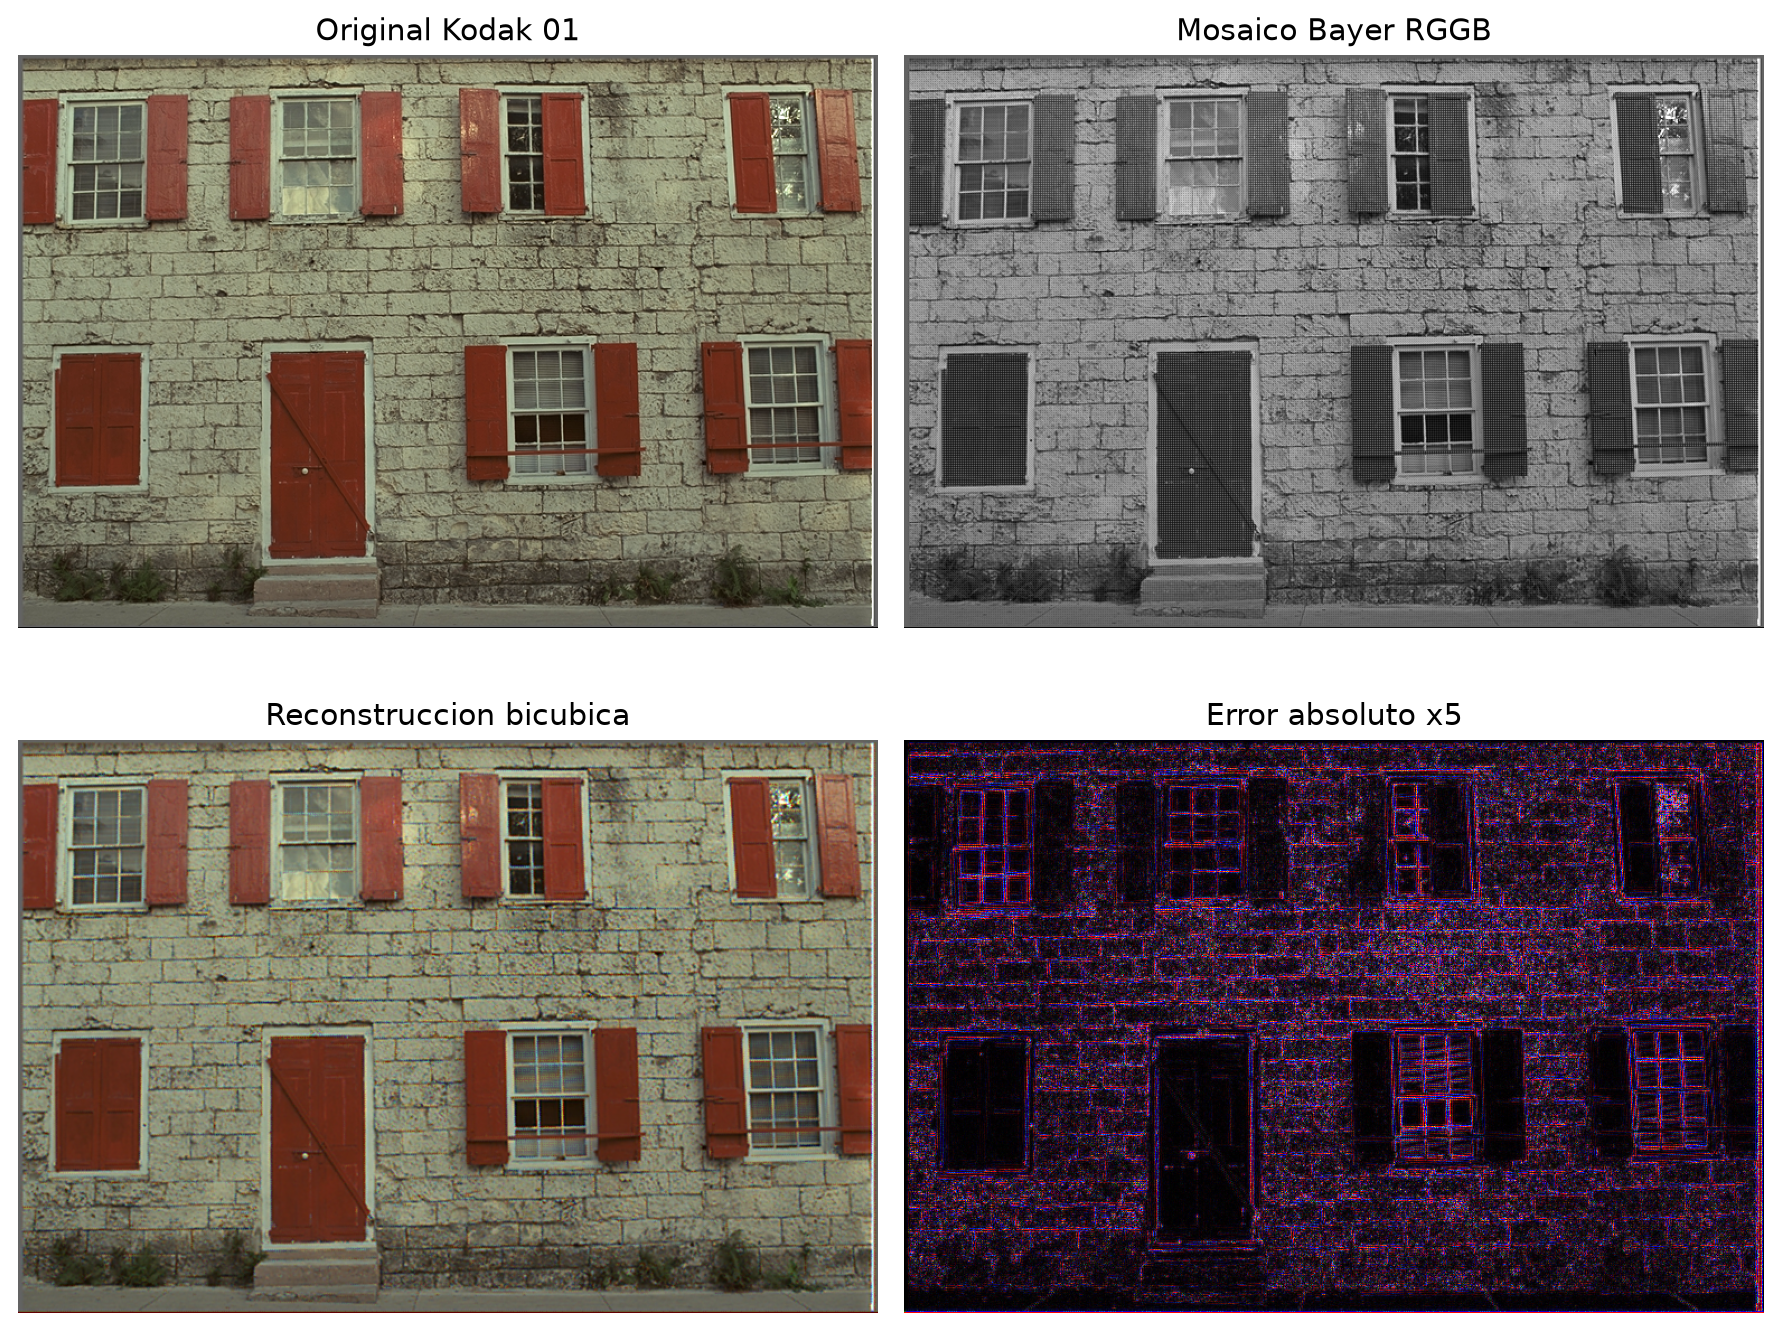
\includegraphics[width=0.92\linewidth]{Fig/kodak01_bayer_bicubica.png}
    \caption{Imagen original, mosaico Bayer RGGB, reconstrucción bicúbica y error absoluto amplificado.}
    \label{fig:bayer_bicubica}
\end{figure}

\subsection{\sffamily Interpolación bicúbica}

La interpolación bicúbica se aplicó de forma independiente a cada canal. Para cada máscara Bayer se tomaron las coordenadas conocidas y sus valores observados; luego se estimaron los valores faltantes sobre toda la grilla espacial mediante interpolación 2D. En los bordes donde la interpolación cúbica puede producir valores no definidos, se usó interpolación por vecino más cercano como respaldo.

\begin{lstlisting}[style=B,caption=Funciones principales para generar el mosaico Bayer e interpolar un canal.,label={lst:bicubica}]
def rgb_to_bayer_mosaic(image_rgb, pattern="RGGB"):
    mask_r, mask_g, mask_b = bayer_masks(image_rgb.shape, pattern=pattern)
    mosaic = np.zeros(image_rgb.shape[:2], dtype=image_rgb.dtype)
    mosaic[mask_r] = image_rgb[..., 0][mask_r]
    mosaic[mask_g] = image_rgb[..., 1][mask_g]
    mosaic[mask_b] = image_rgb[..., 2][mask_b]
    return mosaic

def interpolate_channel(mosaic, mask, method="cubic"):
    height, width = mosaic.shape
    rr, cc = np.indices((height, width))
    known_points = np.column_stack((rr[mask], cc[mask]))
    known_values = mosaic[mask]
    all_points = np.column_stack((rr.ravel(), cc.ravel()))
    channel = griddata(known_points, known_values, all_points,
                       method=method, fill_value=np.nan).reshape(height, width)
    return np.clip(channel, 0.0, 1.0)
\end{lstlisting}

\subsection{\sffamily Bonus: Malvar, He y Cutler 2004}

Además se implementó el algoritmo de Malvar, He y Cutler \cite{malvar2004high}, el cual usa filtros lineales $5 \times 5$ diseñados para reconstruir los canales faltantes en el patrón Bayer. A diferencia de la interpolación bicúbica independiente, este método incorpora correcciones de gradiente y aprovecha mejor la correlación local entre canales, lo que reduce artefactos en bordes, texturas y cambios abruptos de intensidad.

La figura \ref{fig:comparacion_metodos} compara visualmente la reconstrucción bicúbica y Malvar2004 para la imagen 01.

\begin{figure}[!h]
    \centering
    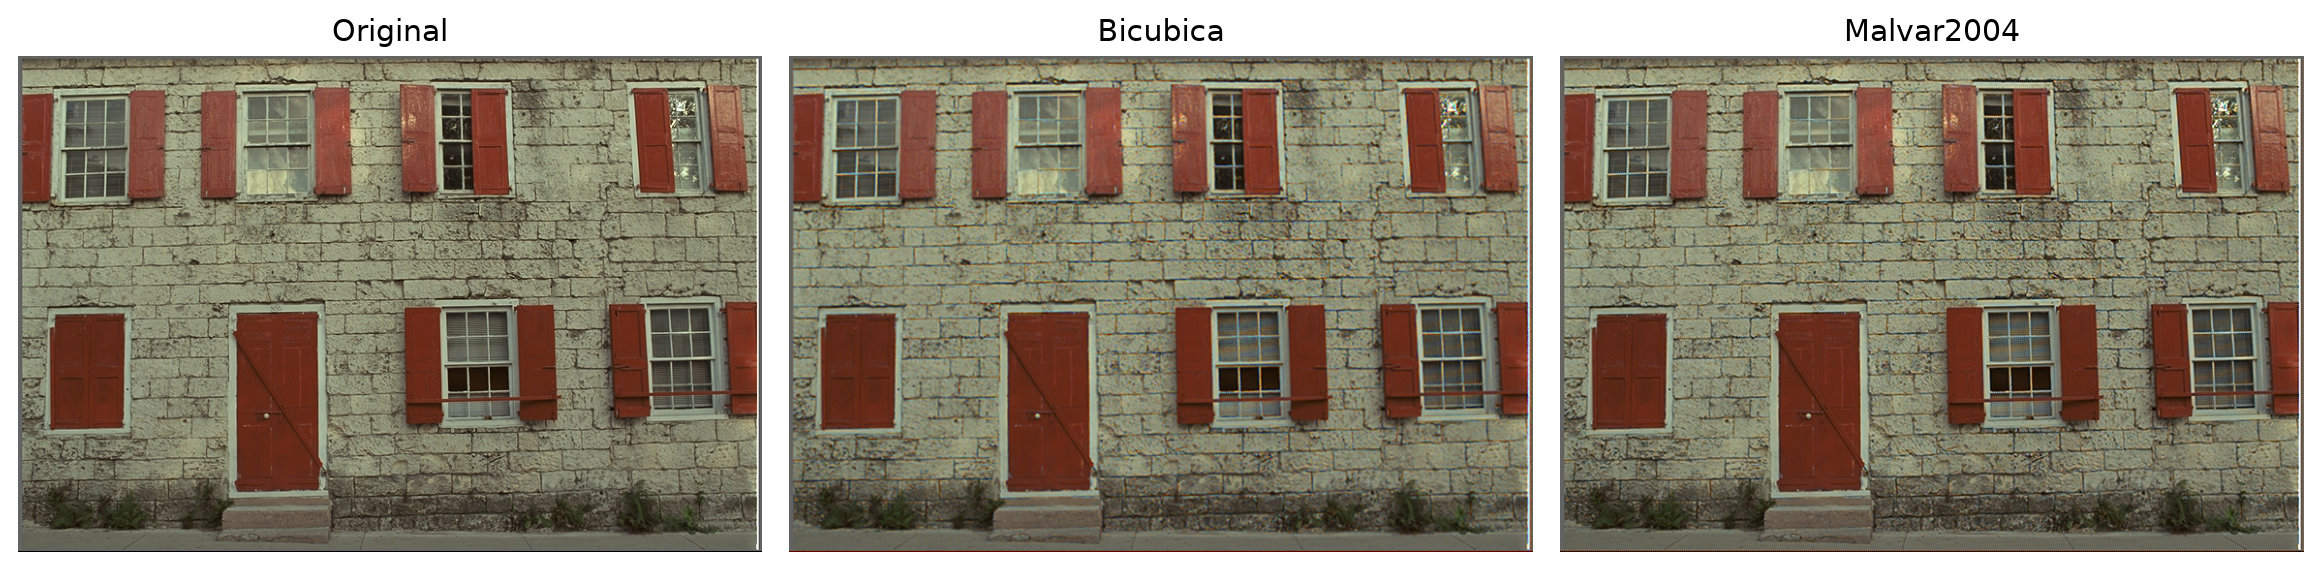
\includegraphics[width=0.95\linewidth]{Fig/kodak01_comparacion_metodos.png}
    \caption{Comparación visual entre imagen original, reconstrucción bicúbica y reconstrucción con Malvar2004.}
    \label{fig:comparacion_metodos}
\end{figure}

\subsection{\sffamily Resultados cuantitativos}

La tabla \ref{tab:resumen_metricas} resume los resultados sobre las 24 imágenes Kodak. En PSNR y SSIM un valor mayor indica mejor reconstrucción, mientras que en SAM un valor menor indica mayor similitud espectral.

\begin{table}[!h]
    \centering
    \caption{Promedio y desviación estándar de las métricas sobre el dataset Kodak.}
    \label{tab:resumen_metricas}
    \begin{tabular}{lrrrrrr}
        \toprule
        Método & PSNR prom. & PSNR std. & SSIM prom. & SSIM std. & SAM prom. & SAM std. \\
        \midrule
        Bicúbica & 29.3046 & 2.9888 & 0.8857 & 0.0425 & 2.7483 & 1.2310 \\
        Malvar2004 & 34.6940 & 2.5837 & 0.9681 & 0.0082 & 1.7049 & 0.6901 \\
        \bottomrule
    \end{tabular}
\end{table}

\begin{figure}[!h]
    \centering
    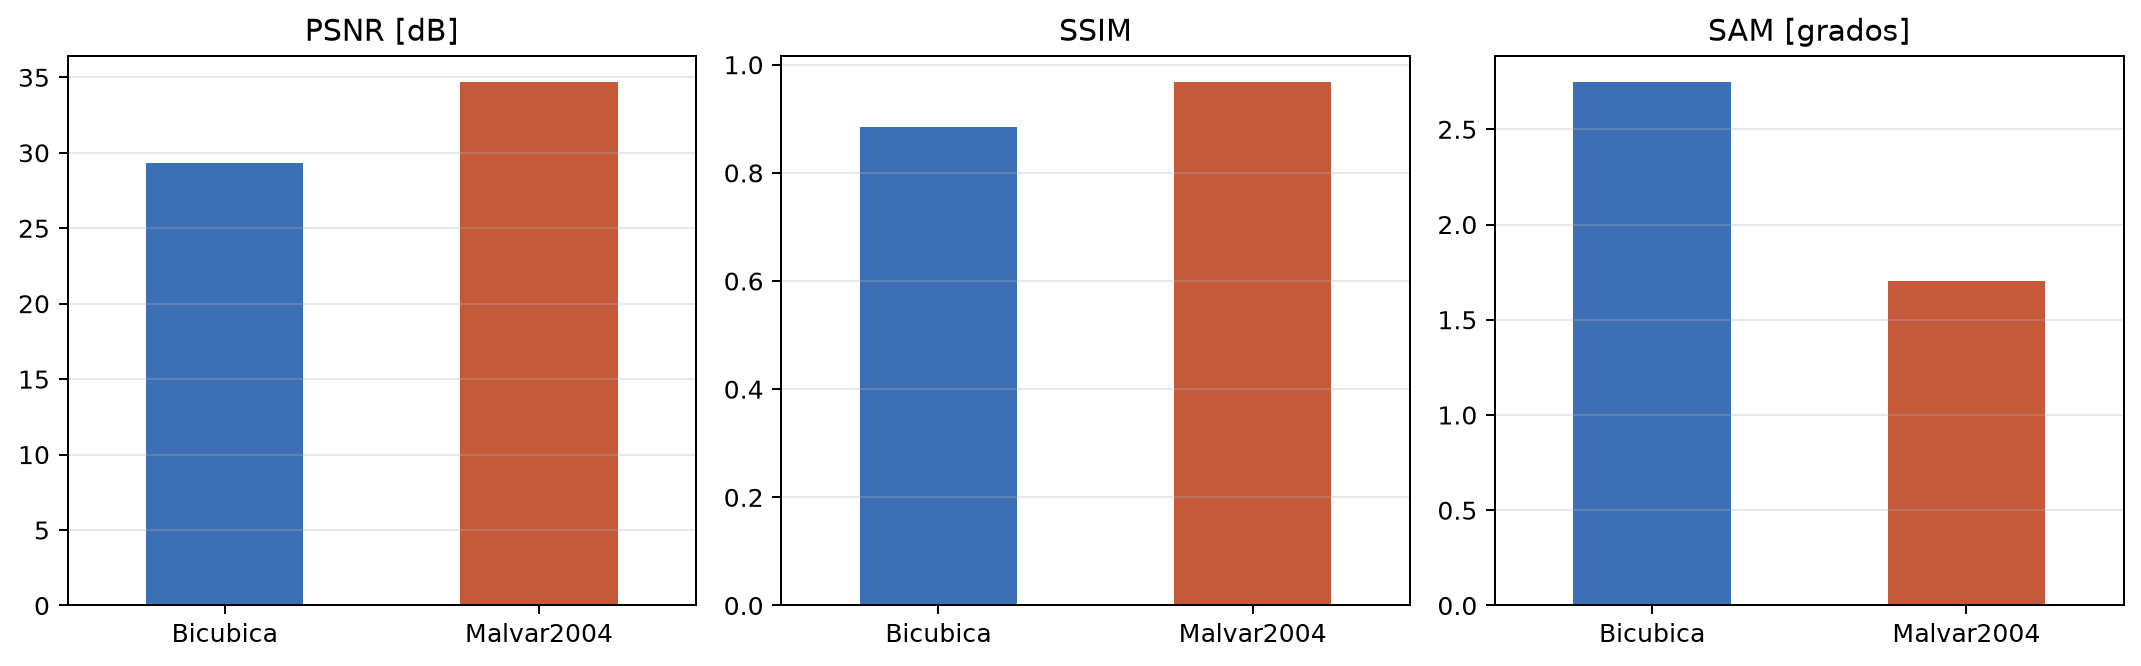
\includegraphics[width=0.9\linewidth]{Fig/comparacion_metricas.png}
    \caption{Comparación de métricas promedio entre interpolación bicúbica y Malvar2004.}
    \label{fig:comparacion_metricas}
\end{figure}

Los resultados por imagen se guardaron en el archivo \texttt{resultados\_metricas.csv}, y el resumen estadístico en \texttt{resultados\_resumen.csv}. Estos archivos se generaron a partir del mismo flujo experimental usado en el notebook.

\section{\sffamily Conclusiones}

Se implementó exitosamente un sistema de fotografía computacional basado en un mosaico Bayer RGGB. La interpolación bicúbica logró reconstrucciones razonables, con un PSNR promedio de 29.3046 dB, SSIM promedio de 0.8857 y SAM promedio de 2.7483 grados. Esto indica que el método conserva buena parte de la estructura visual, aunque presenta limitaciones en bordes y texturas finas debido a que cada canal se interpola de forma independiente.

El algoritmo Malvar2004 obtuvo mejores resultados en todas las métricas: el PSNR promedio aumentó a 34.6940 dB, el SSIM promedio subió a 0.9681 y el SAM promedio bajó a 1.7049 grados. La mejora se explica porque este método usa filtros lineales con corrección de gradiente, incorporando información local y correlación entre canales. Por lo tanto, para el dataset Kodak, Malvar2004 entrega una reconstrucción más precisa y consistente que la interpolación bicúbica independiente.

%-------------------------------------------------------------------------
% BIBLIOGRAPHY
%-------------------------------------------------------------------------

\bibliographystyle{apalike}
\bibliography{Referencias}

\end{document}
